\chapter{Introduction}
\label{chap:intro}

\begin{chapabstract}{Abstract:}
Breast cancer is the second most common cancer worldwide and the leading cause of women's death from cancer. Improving cancer prognosis has been one of the problems of primary interest towards better clinical management and treatment decision making for cancer patients. With the rapid advancement of genomic profiling technologies in the past decades, easy availability of a substantial amount of genomic data for medical research has been motivating the currently popular trend of using computational tools, especially machine learning in the era of data science, to discover molecular biomarkers regarding prognosis improvement. This chapter briefly summarizes the general background of breast cancer with a particular focus on breast cancer prognosis, reviews the prospects and challenges in genomic data analysis, and overviews the methodologies and contribution of the thesis work in this research area.
\end{chapabstract}
\vskip 0.2in
\begin{chapabstract}{R�sum� :}
Le cancer du sein est le deuxi�me cancer le plus r�pandu dans le monde et la principale cause de d�c�s due � un cancer chez les femmes. L'am�lioration du pronostic du cancer a �t� l'une des principales pr�occupations afin de permettre une meilleure gestion et un meilleur traitement clinique des patients. Avec l'avancement rapide des technologies de profilage g�nomique durant ces derni�res d�cennies, la disponibilit� ais�e d'une grande quantit� de donn�es g�nomiques pour la recherche m�dicale a motiv� la tendance actuelle qui consiste � utiliser des outils informatiques tels que l'apprentissage statistique dans le domaine de la science des donn�es afin de d�couvrir les biomarqueurs mol�culaires en lien avec l'am�lioration du pronostic. Ce chapitre r�sume bri�vement le contexte g�n�ral du cancer du sein avec un point particulier sur son pronostic, d�taille les perspectives et les d�fis dans l'analyse des donn�es g�nomiques, et pr�sente les m�thodologies et contributions de la th�se dans ce domaine de recherche.
\end{chapabstract}

\section{General Background of Breast Cancer}

Breast cancer refers to a malignant tumor that has developed from cells in the breast. Uncontrolled growth of cancer cells can invade nearby healthy breast tissue over time, and if cancer cells get into the lymph nodes that are small organs that filter out foreign substances in the body, they could then have a system of spreading further into other parts of the body and form new tumors in distant organs or tissues, a process called distant metastasis that aggravates the situation to a significant extent. Breast cancer is the most common cancer in women worldwide and second most common cancer overall for both genders in terms of incidence rates (following lung cancer), and it is the leading cause of cancer death among women in developing countries and the second leading cause of cancer death (following lung cancer) among women in developed countries \cite{Torre2015Global}.\footnote{See more cancer facts and statistics summary at \url{https://www.cancer.org/research/cancer-facts-statistics.html}.} Over 521,900 women worldwide were estimated to have died in 2012 due to breast cancer \cite{Ferlay2013GLOBOCAN}.\footnote{See more of contemporary estimates of the incidence of, mortality and prevalence from major types of cancer at \url{http://globocan.iarc.fr/}.} Survival rates have in general been improving over the past decades, as a result of increased awareness, earlier detection through mammographic screening, adequate medical care and cancer treatment advances, with the caveat that rates vary greatly worldwide and still remain quite low in less developed countries.


Diagnosis of cancer, determination of the presence (or extent) of the disease, is performed by means of (incisional) \textit{biopsy}, a medical test in which surgeons or interventional cardiologists extract sample cells or tissues for pathologists to examine under microscope or further analyze chemically. If diagnosed early, the initial treatment for breast cancer is usually accomplished by complete removal of tumor by surgery or radiation (mastectomy or less-extensive breast-conserving surgery) without damage to the rest of the body. After the initial treatment (or in case that the initial treatment should not be applicable), many patients receive additional treatment, including adjuvant chemotherapy, hormone therapy and targeted therapy, to lower the risk of relapse, that is the recurrence risk of cancer-related conditions, and/or to prevent metastasis. However, as the most common type of adjuvant therapy, chemotherapy usually involves cytotoxic drugs and has strong deleterious side effects, and the intake of such aggressive treatment should hence be minimized for those that will not necessarily need it. Therefore, to identify those patients who should receive adjuvant chemotherapy is of chief importance in improving the feasibility of treatment deployment in routine clinical management of cancer. The decision of whether to receive such treatment or not is made based on prognosis of the cancer patient, that is the estimation of the risk of relapse or likely course of outcome if no additional treatment is given after the initial treatment, and further treatments are considered most beneficial for patients with poor prognosis and some cases of good prognosis can even choose the option to forgo chemotherapy.\footnote{In fact, two questions need to be addressed in decision making for cancer treatment: prognosis that is the estimation of the course of outcome if no additional treatment is given and hence the identification of those patients who are most likely to need additional treatment; prediction that is the identification of patients who are most likely to benefit from a specific treatment and hence the determination on which treatment should be most responsive and effective for a patient. While prognosis and prediction are equally important and usually discussed together in literature, prediction will be mostly omitted from discussion for ease of the presentation of this thesis.} In order to quantify prognosis results, a patient is usually categorized into prognostic groups of high or low risk corresponding to one of the four common types of survival risk: distant metastasis-free survival, (local or distant) recurrence-free survival, disease-free survival, overall survival. Note that the following discussion applies to any specific survival unless specified otherwise.


Conventionally, breast cancer prognosis is based solely on clinico-pathological information collected of patients and tumors. Several commonly used clinico-pathological parameters have been well-established to be indicative of likely prognosis of patients, and thus widely adopted in the clinical management of breast cancer. For example, it is known that breast cancer with cancer cells detected in lymph nodes has a higher risk of relapse than breast cancer \textit{in situ}, and thus requires to be treated with certain adjuvant chemotherapies that are usually more aggressive \cite{Moffat2014Clinical}. In fact, doctors most often evaluate the severity of breast cancer based on the Nottingham grading system, a score-based grading system using clinico-pathological parameters such as the size and shape of the nucleus in the tumor cells and how many dividing cells are present \cite{Cancer2010AJCC}. High-grade tumors look the most abnormal from normal cells and tend to be the most invasive, and are thus classified with poor prognosis. As another example, hormone receptors in breast cancer, estrogen-receptor (ER) and progesterone-receptor (PR), play an important role in normal glandular development and in breast cancer progression, and their status is therefore highly prognostic (as well as predictive to the responsiveness of hormone and endocrine therapies) \cite{Moffat2014Clinical}. Some online tools exist to perform prognosis of cancer patients and aid physicians weigh against the risks and benefits of adjuvant treatments, among which stands out the renowned \textit{Adjuvant! Online}\footnote{\url{https://www.adjuvantonline.com/}.}. Notably, the six predictors that are shown highly prognostic and used by \textit{Adjuvant! Online} to predict cancer-related mortality and relapse are: patient age, tumor size, grade, hormone receptor status, number of positive lymph nodes and comorbidity level.


Due to the intrinsic heterogeneity across breast cancer tumors, patients of similar clinico-pathological type can have remarkably different survival outcome. An example constituted by \cite{Veer2008Enabling} will be quoted here. Large meta-analyses show that recurrence is likely in 20--30\% of young women with early-stage (lymph node-negative) breast cancer, but in the United States 85--90\% of women with this type of cancer receive adjuvant chemotherapy, among whom 55--75\% therefore undergo a toxic therapy that they would very likely not benefit from but may experience the undesirable side effects. Since cancer is a inherently complex disease, the unwanted situation is mostly due to the fact that clinico-pathological information alone is far from sufficient to reliably identify those patients who are likely to relapse, let alone to accurately characterize the outcome of each particular case in order to personalize the best therapeutic option. It is recognized as an important yet challenging task to improve prognosis for each diseased individual and identify more efficient prognostic features, burgeoning the research of interest in interrogating breast cancer at the molecular level.




\section{Towards Molecular Prognosis}
\label{sec1:molecular}

As \cite{Vogelstein2004Cancer} put it, who are pioneers in cancer molecular biology research:
\begin{quotation}
	\it ``The revolution in cancer research can be summed up in a single sentence: cancer is, in essence, a genetic disease.''
\end{quotation}
Among many theories on cancer biology, a widely accepted theory states that cancer is caused by genomic abnormalities, such as the accumulation of mutations or the dysregulation of gene expression involving tumor suppressor genes and oncogenes in cancer cells. For decades, the number of genes whose involvement in cancer development was established has been increasing significantly, and it has been appreciated that their biological functions are organized by a few principles, named \textit{the hallmarks of cancer}, which rationalize the complexities of cancer and are all underlaid by genome instability generating the genetic diversity \cite{Hanahan2000hallmarks, Hanahan2011Hallmarks}. It is now common knowledge that genomic features contain unique characteristics of each individual being and offer the opportunity of scrutinizing the individuality of each breast tumor. Often termed by \textit{biomarkers} are such molecular features, typically genes, whose abnormal presence or dysfunctional behavior characterizes the biological heterogeneity of tumours, leading to molecular subtyping of cancer, and can thus be indicative of prognosis. While biomarkers can be associated to any phenotype of interest in general, the discussion will particularly focus on biomarkers related to breast cancer prognosis in accordance with the objective of the present thesis.


Many biomarkers related to breast cancer survival have been reported in literature. For example, somatic mutations in gene TP53 show association with worse survival, independent of other risk predictors, see for instance a meta-analysis by \cite{Pharoah1999Somatic}. Worse breast cancer survival of gene BRCA mutation carriers versus non-carriers have been confirmed by several meta-analyses \cite{Zhong2015Effects, Zhu2016BRCA}. Over-expression of gene HER2, pathologically termed as \textit{HER2-positive}, is linked to poorer outcome of node-negative breast cancers \cite{Chia2008Human}, a widely-observed association that has led to the advent of several HER2-directed therapies \cite{Arteaga2012Treatment}. Notably, major molecular subtypes of breast cancer are determined by the gene expression status, over- or under-expression, of hormone receptors and HER2, based on which physicians usually perform prognosis and plan treatments \cite{Schnitt2010Classification}. For a review on currently established and emerging biomarkers for breast cancer prognosis, see \cite{Weigel2010Current}.


From the foundation and completion of Human Genome Project (HGP) to the foundation of The Cancer Genome Atlas Research Network (TCGA), the rapid advancement of genomic profiling technologies in the past decades have paved way to the advent of the current ``omics'' revolution. Nowadays, thousands up to millions of genomic features can be efficiently collected from biological samples available for medical research. Taking gene expression profiling as an example, DNA microarray, a hybridization-based technology, measures the relative expression activity of a large number of predetermined list of target genes in a single experiment (Figure \ref{fig1:microarray}) \cite{Lockhart1996Expression}. RNA-seq, a next-generation sequencing-based technology, was later invented to provide expression measurements of gene sequences at lower cost and higher throughput (or larger genome coverage) with many advantages benchmarked against previous technologies \cite{Wang2009RNA}.

\begin{figure}[!htbp]
\begin{center}

\includegraphics[width=0.9\textwidth]{ch-intro/microarray}
\caption{This image from \cite{Commons2017FileHeatmappng} illustrates an example of gene expression values from microarray experiments represented as a heatmap of two color dyes, with patients in rows and probes in columns, to visualize results of data analysis.}
\label{fig1:microarray}
\end{center}
\end{figure}

The revolution of gene expression profiling technologies fostered the development of multigene expression signatures for breast cancer prognosis, a group of biomarker genes whose combined expression pattern refines prognosis (usually with incremental value added to the use of standard clinico-pathological parameters). The research of prognostic signatures has resulted in many success stories \cite{Sotiriou2009Gene}. Notably, as of today there exist at least six different prognostic multigene expression signatures commercially available to aid clinical decision making of breast cancer:\footnote{See for reference \url{http://www.breastcancer.org/symptoms/testing/types}.}
\begin{bulletList}
	\item MammaPrint\textsuperscript{\textregistered} (Agendia, Amsterdam, The Netherlands) \cite{Veer2002Gene} is a 70-gene microarray-based expression profile for stratifying breast cancer into high- or low-risk prognostic groups. As one of the earliest success stories, it was the first test approved by the Food and Drug Administration (FDA) in the United States and by regulators in the European Union as an adjunct prognostic assay for women patients satisfying criteria\footnote{Indications for ordering an assay can vary in accordance with the clearance issued by the country of application.} including stage I/II, invasive infiltrating carcinoma, tumor size less than 5.0 cm, lymph node negative (or up to three lymph nodes positive).
	\item Prosigna\textsuperscript{\textregistered} Breast Cancer Prognostic Gene Signature Assay or PAM50 (Nanostring Technologies, Seattle, WA, USA) \cite{Parker2009Supervised} is a 50-gene assay for classifying breast tumors into five intrinsic subtypes (luminal A, luminal B, HER2-enriched, basal-like, normal-like) that are prognostic independent of standard clinico-pathological parameters. It is the second FDA-approved test in the United States to estimate distant recurrence risk for stage I/II (including one to three positive nodes), ER-positive breast cancer in postmenopausal women treated with adjuvant endocrine therapy, and it also received clearance in the European Union.
	\item Oncotype DX\textsuperscript{\textregistered} (Genomic Health, Redwood City, CA, USA) \cite{Paik2004multigene} is a 21-gene signature for categorizing tamoxifen-treated breast cancer patients into groups of low-, intermediate- or high-risk recurrence. It is the most widely used prognostic assay for ER-positive cancers in the United States.
	\item MapQuant Dx\textsuperscript{TM} Genomic Grade Index (Ipsogen, France) \cite{Sotiriou2006Gene} is a microarray-based 97-gene assay for reclassifying histologically intermediate-grade ER-positive cancers into high or low molecular grade with significantly different prognosis.
	\item Breast Cancer Index\textsuperscript{SM} (BioTheranostics, San Diego, CA, USA) \cite{Ma2008five} is comprised of two signatures, a 5-gene molecular grade index and the ratio of two independent biomarkers HOXB13:IL17BR, and can assess the risk of distant recurrence in ER-positive, lymph node-negative breast cancers.
	\item EndoPredict\textsuperscript{\textregistered} (Sividon Diagnostics GmbH, Koln, Germany) \cite{Filipits2011new} is a 11-gene signature for stratifying patients with ER-positive cancer into high or low risk of recurrence if treated with adjuvant endocrine therapy alone.
\end{bulletList}
More details about these signatures are found in \cite{Gyorffy2015Multigene}. Notably, another rather famous 76-gene signature (Veridex LLC, a Johnson \& Johnson company, San Diego, CA, USA) \cite{Wang2005Gene} could be used to predict the development of distant metastases within 5 years in lymph node-negative primary breast cancer patients (irrespective of age and tumor size) who did not receive systemic treatment, which was later confirmed in multiple independent studies on patient data obtained from different institutions \cite{Foekens2006Multicenter, Desmedt2007Strong, Zhang200976}.




\section{Genomic Data Analysis: Prospects and Challenges}

In order to study the substantial amount of genomic data available for medical research, the use of computational tools such as machine learning has become a popular trend \cite{Barillot2012Computational}. In fact, machine learning is particularly suitable for analyzing genomic data by developing algorithms or building models to discover unseen patterns, identify complex relationships and predict for phenotypic phenomenon of interest. While genomic data analysis of cancer is a research field encompassing a broad range of topics, the present thesis is specifically devoted to breast cancer prognosis and related biomarker discovery. In the language of machine learning, \textit{cancer prognosis} is usually formulated as \textit{predictive modeling} (or discriminative modeling succeeding supervised learning) and \textit{biomarker discovery} is formalized as \textit{feature selection}. In fact, an extensive body of findings in the genre of genomic data analysis are inferred from empirical evidence of relationship between the genomic features and the survival information collected over large population of patients. Given a set of $m$ observations $\mathcal{D} := \{ (\xb_1 , y_1), \dots, (\xb_m , y_m) \},$ where $\xb_i \in \XX$ denotes the feature vector of the $i$-th sample, typically the expression measurements of $n$ genes (or $i$-th row in Figure \ref{fig1:microarray}\footnote{Probes are hybridization fragments of DNA, therefore probe-specific measurements in microarray data usually need post-processing to estimate gene-specific measurements.}) in gene expression data analysis when $\XX = \RR^n$, and $y_i \in \YY$ denotes the outcome of the $i$-th sample, typically the survival time when $\YY = \RR \times \{0,1\}$ of (positive) survival observation with a right-censoring flag, or the prognostic group when $\YY = \{1,\dots,K\}$ of $K \geq 2$ groups categorized by thresholding the observed survival time, the objective is then to infer a predictive function $h : \XX \to \YY$ which can then be used to predict survival risk or classify prognostic group for any new sample. These two learning tasks are termed respectively as \textit{survival analysis} and \textit{classification} in machine learning literature.


Survival analysis is generally referred to a set of methods for analyzing data where the outcome variable is the time until the occurrence of an event of interest, hereby referring to the survival time when $\YY = \RR \times \{0,1\}$. In clinical management of cancer, patients are usually followed for a specified time period and the focus is on the time at which the event of interest occurs such as metastasis, recurrence or death. If the event had occurred during the follow-up, the survival time is documented by the observed time to event; if the event had not occurred by the end of the follow-up (or the patient dropped out of the study), the event had not yet been observed and the survival time is documented by the follow-up (or drop-out) time with a flag, meaning that survival time can only be considered at least as long as the duration of follow-up. A survival observation is called right-censored if it is incomplete as in the latter case. Survival time is therefore a variable consisting of two components: the documented survival time (usually measured in days) and a right-censoring flag indicating whether the survival is exact or lower-bounded, leading to $\YY = \RR \times \{0,1\}$ in survival analysis. A number of methods are available in literature to analyze the relationship of the feature vector with the survival time, among which two are worth special mention. Kaplan-Meier method \cite{Kaplan1958Nonparametric} is a nonparametric estimator and graphical method of depicting survival probabilities as a function of time. It is widely used to obtain descriptive statistics for survival observations that can be further combined with statistical tests to compare the survival experience for two or more groups of patients\footnote{Patients are usually grouped by molecular subtypes typically by clustering approaches based on their genomic features.}. Cox proportional hazards model \cite{Cox1972Regression} is a popular regression model for analyzing survival data that builds an easily interpretable model associating the relationship of the survival hazards to predictive features in order to describe the likely course of outcome. For a textbook-oriented overview of survival analysis, see \cite{Hosmer1999Applied}.


Classification is another classical topic in machine learning and statistics where the outcome variable belongs to one of a few predetermined categories, specifically $\YY =  = \{1,\dots,K\}$ representing $K \geq 2$ prognostic groups. Based on their clinical records of survival time, cancer patients can be categorized into high-risk and low-risk (and sometimes a third intermediate-risk) groups typically by binarizing the continuous survival time at a 5-year threshold. In fact, deployment of cancer treatment usually relies on such manageable categorization of patients into prognostic groups. Compared to survival analysis, classification bypasses the difficulty in accurately depicting the course of survival outcome but instead seeks a coarse yet clinically meaningful description of survival outcome. Popular classification methods include Fisher's linear discriminant \cite{Fisher1936use}, logistic regression \cite{Cox1958Regression}, decision trees \cite{Breiman1984Classification}, Support Vector Machines \cite{Cortes1995Support}, Random Forests \cite{Breiman2001Random}, Gradient Boosting Machines \cite{Friedman2001Greedy}, see \cite{Hastie2009Elements} for details and many other algorithms for classification.


The predictive modeling framework discussed above assumes that a representation of all sample vectors consisting of $n$ genomic features is already determined and will be included in building a predictive model. In the era where we have easy access to thousands up to millions of genomic features for a biological sample albeit most of which can be irrelevant or redundant for the inference task under consideration, it is crucial to determine which features to be incorporated in the model, a question usually termed as \textit{feature selection} in machine learning or \textit{biomarker discovery} in computational biology. On one hand, inferring a predictive model with a large number of features from a relatively small number of samples, which is usually the case in biomedical applications, is essentially difficult from the viewpoint of statistical inference, a phenomenon referred to as \textit{the curse of dimensionality}, which often leads to unreliable models that overfit the observed samples and generalize poorly when used to predict for future samples. Reducing the number of features representing each sample by selecting only a few important features has proven an efficient way to limit this difficulty.\footnote{Besides feature selection, another efficient approach of dimensionality reduction is via feature extraction such as principal component analysis. While feature selection finds a subset of informative features \textit{as is} without altering the original representation of data, feature extraction transforms the data in the high-dimensional feature space to a space of lower dimension.} On another hand, the identification of a few informative genomic features helps suggest discerning interpretation and key insights into molecular cancer biology. Further, a few identified biomarkers can facilitate the design of more affordable prognostic gene signatures as it is still cheaper and faster to measure the activity of a few targeted genes nowadays.


Many feature selection techniques exist and are organized into three categories, depending on how they are combined with the construction of the predictive model: filter methods, wrapper methods and embedded methods. (Univariate) filter methods select a list of relevant features from the entire feature set independent from the predictive models used, by assessing the relevance of each feature to the response of interest with an importance score, typically by applying some statistical test such as $\chi^2$-test or calculating some information measure univariately such as Information Gain \cite{Xing2001Feature}, and removing those low-scoring ones. Being the computationally fastest methods, filter methods can easily scale to a large number of features and accommodate any predictive model, whereas they usually ignore the interaction between features and special attributes of the predictive model considered. Taking into account the dependencies between features and the hypothesis of the predictive model, wrapper methods aim to directly find the best combination of features by evaluating all possible feature subsets as input to the model and picking the one with which the resulting model performs the best. Due to the fact that the space of feature subsets grows exponentially with the number of features, exhaustive search over the full space of feature subsets is in general computationally impossible, and hence heuristic or greedy algorithms are often adopted to guide the search for a satisfactory candidate of feature subset. Popular wrapper methods include simulated annealing \cite{Kirkpatrick1983Optimization} and sequential elimination such as stepwise regression \cite{Hocking1976analysis}. Embedded methods enable feature selection during the process of constructing a predictive model, and as these methods are usually tailored to each specific model utilized, they are therefore far less computationally intensive than wrapper methods. Popular embedded methods include a wealth of regularization methods such as the lasso \cite{Hastie2009Elements} and recursive feature elimination embedded in Support Vector Machines \cite{Guyon2002Gene}. For an overview of feature selection methods, see \cite{Guyon2003introduction, Li2016Feature} for an introductory review from the methodological viewpoint of machine learning and \cite{Saeys2007review, Hira2015review} with a particular emphasis on applications in bioinformatics.


While survival analysis, classification and feature selection are themselves extensively studied and still active research areas of machine learning research, their applications in genomic data analysis are a particularly demanding task. In fact, it has been widely recognized as a challenging problem to extract potentially valuable information from genomic data for reasons of multiple folds. To start with, cancer is intrinsically a highly complex disease and consequently the heterogeneity underlying cancer patients renders inevitable obstacle in analyzing cancer data, in other words, high-throughput experimental data are noisy by nature leading to a decline in the informativeness of such data. In addition, from the viewpoint of machine learning, a relatively small number of clinical samples (typically at the scale of $10^2 \sim 10^3$) versus a large number of genomic features (typically at the scale of $10^3 \sim 10^6$) adds difficulty in making reliable inference from analyzing observed samples that could generalize well to future samples and in identifying prognostic biomarkers reusable for future patients. Another major concern specially regarding biomarker discovery is the \textit{a posteriori} interpretation of the computational findings in terms of biological relevance to the mechanism of cancer. To address the challenges in genomic data analysis, there is a pressing need for bioinformatics-oriented methods built upon state-of-the-art machine learning algorithms as a stepping stone.


Despite the computational challenges confronted by machine learning applications in cancer prognosis, many success stories are prominent. For example, the above-mentioned PAM50 test, the 50-gene classifier for subtyping breast cancer, is constructed upon a learning algorithm called the nearest shrunken centroid method \cite{Tibshirani2002Diagnosis}. Another example comes from the \textit{DREAM 7 --- Sage Bionetworks--DREAM Breast Cancer Prognosis Challenge} \cite{Margolin2013Systematic}, a competition-based crowd-source effort that systematically assessed and confirmed the potential of computational models designed to predict breast cancer survival by combining various types of molecular features with standard clinico-pathological parameters to improve prognosis performance (Figure \ref{fig1:competition}) \cite{Bilal2013Improving}. Notably, the best-performing model of the competition \cite{Cheng2013Development} was built upon, in addition to clinico-pathological features, such molecular features called \textit{attractor metagenes} that are pan-cancer signatures of coexpressed genes previously identified in rich gene expression datasets by an iterative attractor-finding algorithm \cite{Cheng2013Biomolecular}. For a recent survey on machine learning applications in cancer prognosis, see \cite{Kourou2015Machine}. Worth special mention are two lines of ideas to address the difficulty in cancer prognosis and biomarker discovery, which have primarily motivated the work presented in this thesis.


\begin{figure}[!htbp]
\begin{center}
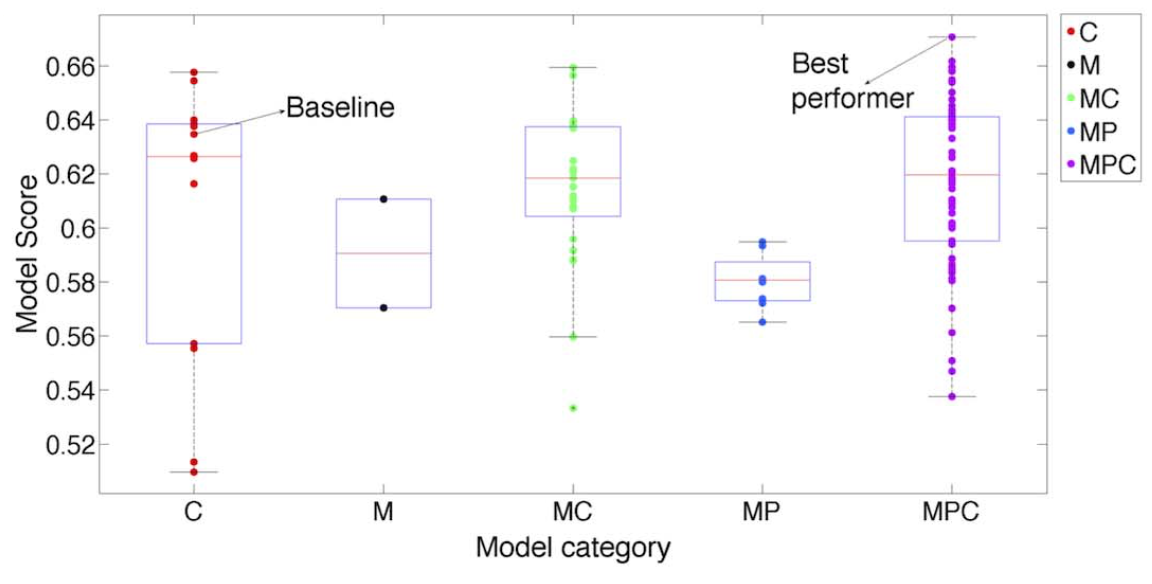
\includegraphics[width=0.9\textwidth]{ch-intro/competition}
\caption{This figure from \cite[Figure 2]{Bilal2013Improving} illustrates that the best performer among submissions to the pilot competition uses a combination of clinical and molecular features that are deliberately selected subject to prior knowledge (the MPC category). Models submitted are categorized by the type of features they use: only clinical features (C), only molecular features (M), molecular and clinical features (MC), molecular features selected using prior knowledge (MP), molecular features selected using prior knowledge and clinical features (MPC).}
\label{fig1:competition}
\end{center}
\end{figure}


Since high-throughput high-dimensional gene expression data are often subject to high measurement noise, the ranking of the expression levels of multiple genes are presumably more robust predictors, in the sense that they can be less sensitive to noise, than their real-valued measurements. This can be particularly beneficial in many biomedical applications when the informativeness (or signal-to-noise ratio) in data is low. Pioneering the exploration of these ideas is the top scoring pairs (TSP) \cite{Geman2004Classifying}, an algorithm for classifying gene expression profiles by pairwise microarray comparison, together with successive extensions and further investigations by \cite{Tan2005Simple, Xu2005Robust, Lin2009ordering}. These methods generate simple and accurate decision rules to discriminate cancer samples from normal ones based on the relative reversals of pairwise ordering comparing the expression of a few genes. However, when it comes to biomedical classification on difficult tasks such as cancer prognosis that usually involves the collaborative functional activities of a relatively large number of gene, the performance of TSP-family classifiers degrades drastically, probably due to the naively simple majority voting scheme adopted by those classifiers. In order to improve cancer outcome prediction, many studies employed TSP algorithm as a feature selection technique that is further embedded into more complex classification methods such as Support Vector Machines \cite{Shi2011Top} or decision trees \cite{Czajkowski2011Top} in microarry data analysis.


Cancer is a ``network disease''. In fact, it has already been quoted above that cancer is a genetic disease. As more and more cancer-related genes were identified and arranged into signaling pathways through which they act, it became apparent that these pathways are interconnected and present crossroads at different levels \cite{Vogelstein2004Cancer}, indicating that tumor progression is the consequence of network-level dysregulation of interactions between genes, RNAs, proteins and other molecules that control at least the hallmarks of cancer \cite{Hanahan2011Hallmarks}. Moreover, biological networks, including protein-protein interaction, coexpression and regulatory networks, or metabolic and signaling pathways, are a common way of depicting functional relationships between genes that have been accumulated from decades of biomedical research, and they can be potentially valuable when incorporated as domain-specific knowledge during the process of the computational analysis of genomic data so as to, for instance, improve stability and interpretability of biomarker discovery (Figure \ref{fig1:network}). Approaches to pathway and network analysis techniques range broadly, including gene set enrichment analysis that identifies genes of interest appearing in pathways more frequently than expected by chance \cite{Subramanian2005Gene}, network modeling that infers the activities and interactions of various genetic components in pathway or networks, see for instance \cite{Tarca2008novel, Drier2013Pathway, Vandin2011Algorithms, Hidalgo2017High}, network-guided predictive modeling that consults the structure of \textit{a priori} known network and constrains the predictive modeling procedures discussed above so that the ``ideal'' model or biomarkers selected should be coherent with the network, see for instance \cite{Li2010Variable, Rapaport2007Classification, Jacob2009Group}. For a recent review of pathway and network analysis of cancer genomes, see \cite{Creixell2015Pathway} with a focus on approaches applied to somatic single nucleotide variants (SNVs) and altered RNA expression and \cite{Azencott2016Network} with a particular emphasis on biomarker discovery.


\begin{figure}[!htbp]
\begin{center}
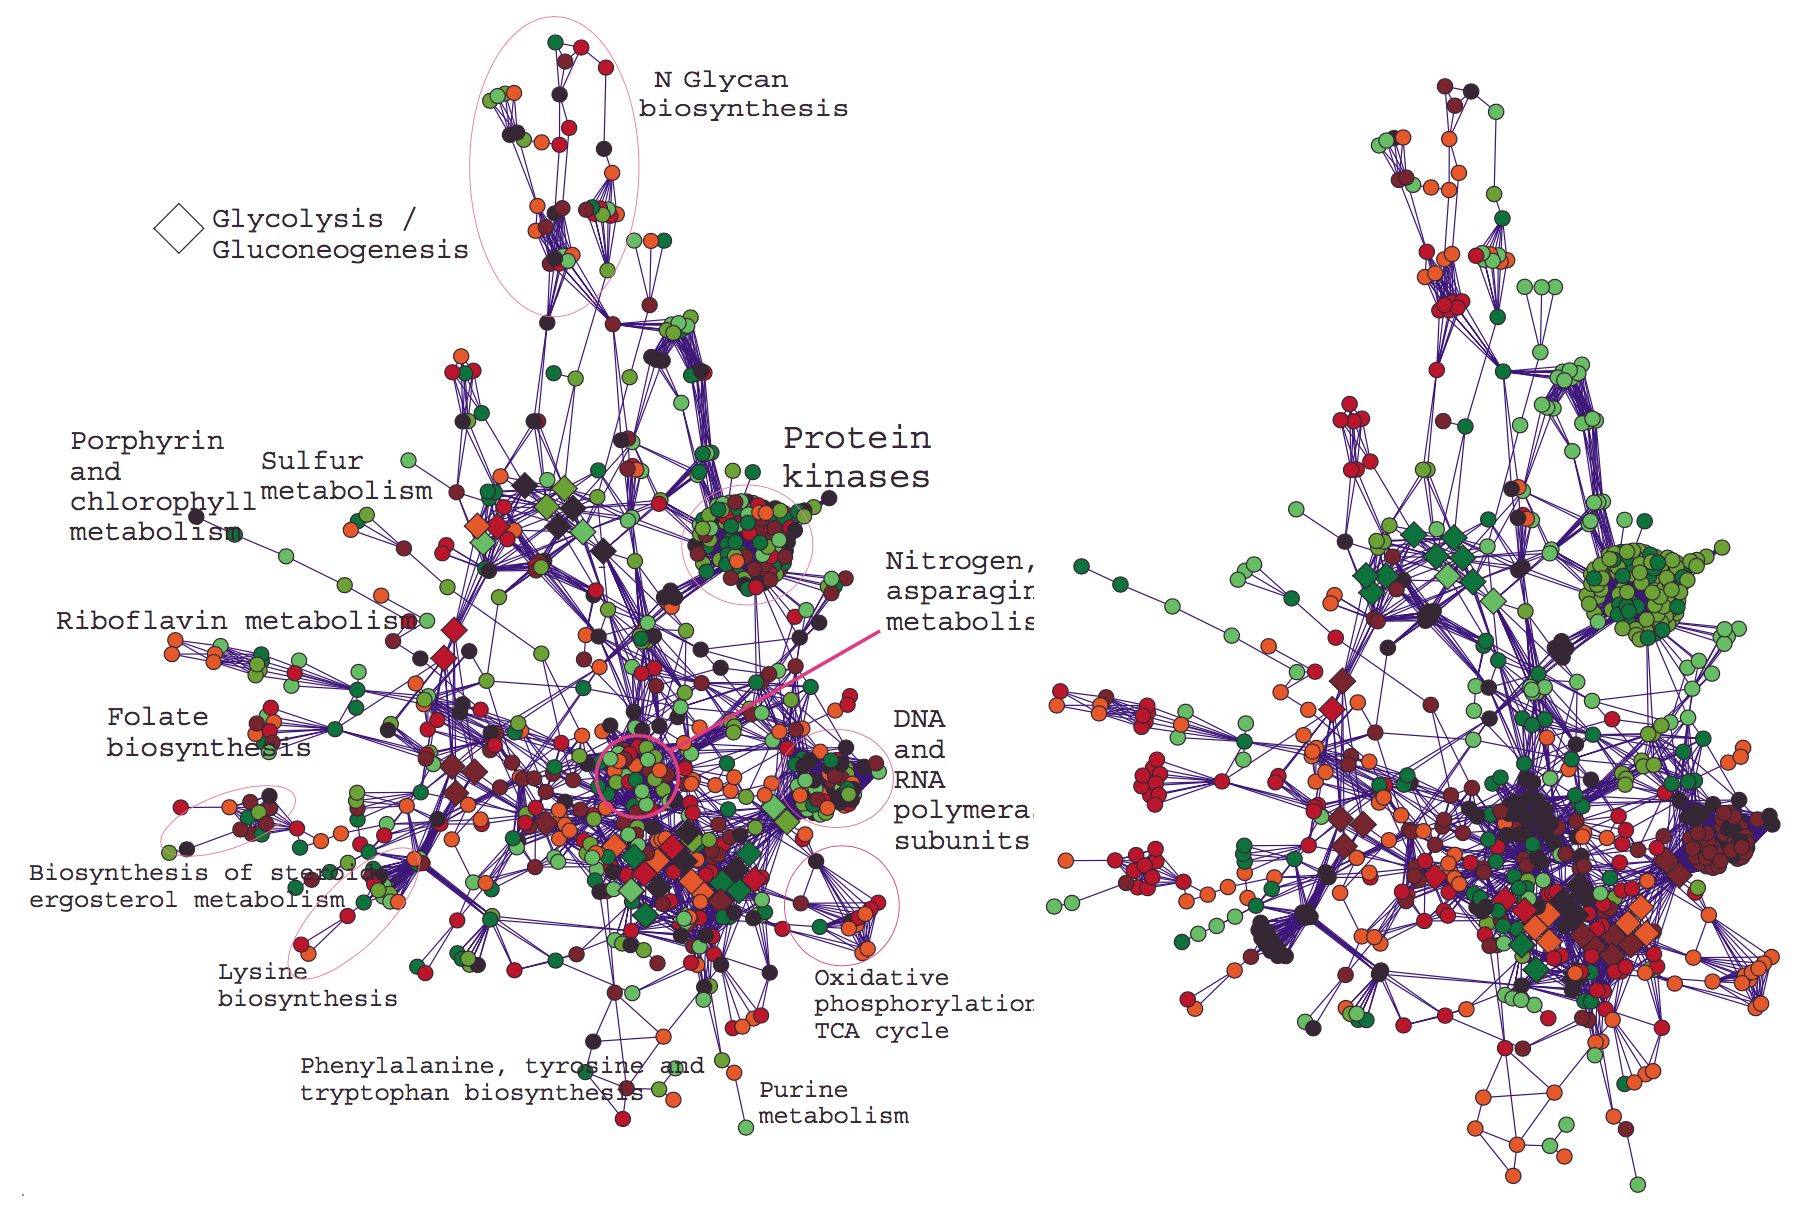
\includegraphics[width=0.9\textwidth]{ch-intro/network}
\caption{This figure from \cite[Figure 3]{Rapaport2007Classification} illustrates an example of metabolic pathways, mapped by coefficients of the decision function obtained by applying a network-free model (left) and a network-guided model (right) in color, positive in red and negative in green with intensities reflecting absolute values, where some large highly connected functional parts of the network with annotations such as proteinkinases and DNA and RNA polymerase subunits were identified by the network-guided model, rendering readily available interpretability to the involvement of the selected genes in cancer.}
\label{fig1:network}
\end{center}
\end{figure}


\section{Contribution of the Thesis}

The thesis work is conceived following the two lines of ideas intended to address two major questions from the methodological standpoint of machine learning: rank-based approaches for improved molecular prognosis and network-guided approaches for enhanced biomarker discovery. Furthermore, despite their biomedical application in cancer prognosis to which this thesis is largely devoted, the methodologies developed and investigated in this thesis, pertaining respectively to learning with rank data and learning on graphs, have a significant contribution to several branches of machine learning, concerning applications across but not limited to cancer biology and social choice theory. This thesis will be organized by projects, each presented in one chapter.


\subsection{Rank-based Approaches for Improved Molecular Prognosis}

The first line of ideas is to perform gene expression data analysis based on exploiting exclusively the ranking of the expression levels of multiple genes while their real-valued measurements are disregarded, which integrates the idea of relative reversals of pairwise ordering inherited from TSP-family classifiers in the paradigm of kernel learning. From the point view of machine learning, the problem reduces to the study of a particular type of structured data, specifically rankings. It is well-known that kernel methods have found many successful applications where the input data are discrete or structured including strings and graphs \cite{Gaertner2004Kernels}. The first project of my doctoral studies was focused on proposing computationally attractive kernels for rank data and applying kernel methods to problems involving rankings. Central to this work was the observation that the widely used Kendall tau correlation and the Mallows similarity measure are indeed positive definite kernels for total rankings. These kernels were further tailored to more complex types of rank data that prevail in real-world applications, especially uncertain rankings which are converted from real-valued vectors by keeping simply the relative ordering of the values of multiple features thereof. Thanks to these kernels, many off-the-shelf kernel machines are available to solve various problems at hand \cite{Shawe-Taylor2004Kernel, Schoelkopf2004Kernel}. It is worth special mention that, despite that the project was initially motivated by biomedical applications, the prospective contribution of this work concerns applications from many fields of machine learning pertaining to learning from rankings, or learning to rank. This study will be presented in Chapter \ref{chap:kendall}.


The study of the Kendall kernel for rankings has paved an unprecedented way towards a deeper understanding of a classical problem called Kemeny aggregation \cite{Kemeny1959Mathematics} from the field of social choice theory. Kemeny aggregation searches for a consensus ranking that best represents a collection of individual rankings in the sense that the sum of the Kendall tau distance between each ranking and the consensus is minimized. Although Kemeny aggregation is often considered to provide the ``golden'' solution among all ranking aggregation criteria, the Kemeny consensus is known to be NP-hard to find \cite{BartholdiIII1989Voting}. Many tractable approximations to the Kemeny consensus have therefore been proposed and extensively studied, see for instance \cite{Ali2012Experiments}. Since the Kendall kernel derives from an inner product of a Euclidean space, the Kendall tau distance derives from a squared Euclidean distance. As a result, the combinatorial problem of Kemeny aggregation is endowed with an intuitive interpretation from a geometric point of view. Based on this observation, a tractable upper bound of the estimation error in terms of the distance between the exact Kemeny consensus and an approximate solution is established. This upper bound requires little assumption on the approximation procedure or the collection of rankings to aggregate. Due to its remote connection to cancer prognosis or the primary objective of this thesis, this study will be presented in Appendix \ref{chap:kemeny}.


\subsection{Network-guided Approaches for Enhanced Biomarker Discovery}

The second line of ideas of performing genomic data analysis for cancer prognosis is to consult biological networks as prior knowledge in order to improve the selection efficacy of molecular features. Two projects were initiated on network-guided analysis of genomic data for suggesting candidate biomarkers related to cancer prognosis.


In one project, we focused on the study of structured regularization in generalized linear models \cite{McCullagh1989Generalized} and the Cox proportional hazards model \cite{Cox1972Regression} where the regularization method is designed so that genes closer on the biological network are encouraged to be selected simultaneously as candidate biomarkers. In fact, in order to achieve simultaneous modularity and sparsity coherent with the presumed network structure, a popular method called network-based wavelet smoothing has been successfully applied in many applications from the field of signal processing \cite{Shuman2013emerging}. Therefore, we were intrigued to investigate the potential of this method in survival analysis of breast cancer with a gene expression dataset guided by a protein-protein interaction network, albeit the methodology is generally applicable to various types of genomic data and biological networks. In particular, the method allows to designate genes as candidates for biomarkers in form of gene modules with intra-collaborative functionality rendering readily interpretable insights related to cancer survival. Numerical results demonstrated that, compared to several network-free and some established network-based regularization methods, network-based wavelet smoothing was able to improve the selection efficacy of genes related to cancer survival in terms of stability, connectivity and interpretability, while achieving competitive performance of survival risk prediction. This study will be presented in Chapter \ref{chap:wavelet}.


In another project, we focused on a particular type of biological network namely signaling pathway network. Based on a modeling framework of cell signaling proposed by \cite{Hidalgo2017High}, gene expression profiles can be translated into personalized profiles of signaling pathway activities by integrating known signaling pathways. When gene-level profiles are replaced by these derived pathway-level profiles as input to many off-the-shelf computational tools, a simple scheme emerges where gene-level analysis is easily promoted to pathway-level analysis of gene expression data. The advantage is remarkable in that, when combined with feature selection methods, the proposed scheme enables direct identification of pathway-level mechanistic signatures as an alternative to conventional gene-based signatures, which provides more informative insights into the cellular functions and biological processes involved in cancer. This study will be presented in Chapter \ref{chap:hipathia}.


\subsection{Other Contributions}

During the course of my doctoral studies, I have undertaken some other projects as well. In 2013, Elsa Bernard, Erwan Scornet, V\'{e}ronique Stoven, Thomas Walter, Jean-Philippe Vert from our laboratory and I participated in the \textit{DREAM 8 NIEHS--NCATS--UNC Toxicogenetics Challenge}, an international bioinformatics competition where participants were asked to predict the response of human cell lines exposed to various toxic chemical compounds based on the molecular characterization of chemicals and the transcriptome of cell lines. Finally our team won second place with a kernel bilinear regression model. Oral presentation was accepted to \textit{NIPS Workshop on Machine Learning in Computational Biology (MLCB)} and later invited to \textit{RECOMB Conference on Regulatory and Systems Genomics}. This work has been published as part of the crowd-source collaboration as a result of the competition \cite{Eduati2015Prediction} but will be excluded from this thesis.


During my internship at Roche Diagnostics GmbH, Penzberg, Germany, I worked on failure state prediction for automated analyzers for analyzing biological samples in collaboration with Jean-Philippe Vert, Fabian Heinemann, Sven Dahlmanns and Stefan Kobel, and a European patent regarding the application was filed by Roche Diagnostics GmbH, F. Hoffmann--La Roche AG in December 2016 and is currently pending approval \cite{Jiao2016Failure}. Due to corporate confidentiality policies, this study will not be included in this thesis.
